\documentclass[12pt]{article}
\usepackage[utf8]{inputenc}
\usepackage[margin=1in]{geometry}
\usepackage{amsmath,amssymb}
\usepackage{graphicx}
\usepackage{hyperref}
\usepackage{enumitem}
\usepackage{fancyhdr}
\usepackage{tikz}
\usetikzlibrary{shapes,arrows,positioning}

\pagestyle{fancy}
\fancyhf{}
\rhead{Patent Application}
\lhead{Coherence-Based Anesthesia}
\rfoot{Page \thepage}

\title{\textbf{METHODS AND SYSTEMS FOR COHERENCE-BASED\\ANESTHESIA MONITORING AND DRUG DESIGN}\\[1em]
\large Provisional Patent Application}

\author{Jonathan Washburn\\
\texttt{washburn.jonathan@gmail.com}}

\date{January 18, 2026}

\begin{document}

\maketitle

\begin{center}
\textbf{PROVISIONAL PATENT APPLICATION}\\[0.5em]
Filed under 35 U.S.C. \S 111(b)
\end{center}

\vspace{1em}

\tableofcontents
\newpage

%==============================================================================
\section{TITLE OF THE INVENTION}
%==============================================================================

\textbf{Methods and Systems for Coherence-Based Anesthesia Monitoring, Depth Assessment, and Rational Anesthetic Drug Design Using Recognition Science Principles}

%==============================================================================
\section{CROSS-REFERENCE TO RELATED APPLICATIONS}
%==============================================================================

This application claims the benefit of theoretical foundations established in Recognition Science (RS), including the Gap-45 coherence threshold and 8-tick neural synchronization mechanisms.

%==============================================================================
\section{FIELD OF THE INVENTION}
%==============================================================================

The present invention relates to anesthesiology, neuroscience, and pharmaceutical design. More specifically, it relates to:

\begin{enumerate}[label=(\alph*)]
    \item Methods for monitoring anesthesia depth using coherence-based metrics
    \item Systems for real-time assessment of consciousness during surgery
    \item Rational design of safer anesthetic drugs based on coherence disruption principles
    \item Algorithms for predicting emergence timing from anesthesia
    \item Devices for measuring neural coherence in clinical settings
\end{enumerate}

%==============================================================================
\section{BACKGROUND OF THE INVENTION}
%==============================================================================

\subsection{The Problem of Anesthesia Monitoring}

General anesthesia has been used clinically since 1846, yet the mechanism by which anesthetics cause unconsciousness remains incompletely understood. Current monitoring methods include:

\begin{itemize}
    \item \textbf{BIS (Bispectral Index)}: EEG-based, correlates with depth but mechanism unclear
    \item \textbf{Entropy monitoring}: Measures EEG entropy, empirical correlation
    \item \textbf{MAC (Minimum Alveolar Concentration)}: Dose-based, population average
    \item \textbf{Clinical signs}: Heart rate, blood pressure, movement (unreliable)
\end{itemize}

These methods are empirical and do not address the fundamental question: \textit{what is the mechanism of anesthetic-induced unconsciousness?}

\subsection{The Recognition Science Framework}

Recognition Science (RS) provides a theoretical framework that explains consciousness as emerging from \textbf{coherent recognition} across neural populations. Key concepts include:

\begin{itemize}
    \item \textbf{Gap-45}: The threshold separating quantum and classical domains ($\sim 10^{45}$)
    \item \textbf{8-Tick Synchronization}: The fundamental timing cycle for neural binding
    \item \textbf{J-Cost}: The recognition cost function governing state selection
    \item \textbf{Coherence}: The degree of synchronized recognition across brain regions
\end{itemize}

Under this framework, \textbf{anesthetics work by disrupting coherence}, thereby preventing the integrated recognition that constitutes consciousness.

\subsection{Prior Art Limitations}

Existing anesthesia monitoring systems:
\begin{enumerate}
    \item Lack mechanistic basis for their measurements
    \item Cannot predict individual patient responses
    \item Have significant false positive/negative rates
    \item Cannot guide drug design rationally
\end{enumerate}

The present invention addresses these limitations by providing a \textbf{first-principles approach} to anesthesia based on coherence disruption.

%==============================================================================
\section{SUMMARY OF THE INVENTION}
%==============================================================================

The present invention provides:

\subsection{Core Innovation}

A method for assessing anesthetic depth by measuring \textbf{neural coherence} as defined by Recognition Science, where:

\begin{equation}
\text{Consciousness State} = f(\text{Coherence Level}, \text{Gap-45 Threshold})
\end{equation}

Specifically:
\begin{itemize}
    \item Coherence above threshold $\rightarrow$ Conscious
    \item Coherence below threshold $\rightarrow$ Unconscious
    \item Coherence at threshold $\rightarrow$ Transitional (high awareness risk)
\end{itemize}

\subsection{Key Claims Preview}

\begin{enumerate}
    \item Method for monitoring anesthesia depth using coherence metrics
    \item System for real-time coherence measurement and display
    \item Algorithm for predicting emergence timing
    \item Method for designing anesthetics targeting coherence disruption
    \item Device for measuring 8-tick synchronization across brain regions
\end{enumerate}

%==============================================================================
\section{DETAILED DESCRIPTION OF THE INVENTION}
%==============================================================================

\subsection{Theoretical Foundation: The Coherence Model of Anesthesia}

\subsubsection{The Gap-45 Threshold}

In Recognition Science, consciousness emerges when neural coherence exceeds a critical threshold related to the Gap-45 value ($\sim 10^{45}$). This threshold separates:

\begin{itemize}
    \item \textbf{Quantum regime}: Superpositions, delocalized states
    \item \textbf{Classical regime}: Definite states, localized recognition
    \item \textbf{Consciousness}: Coherent integration at the boundary
\end{itemize}

\subsubsection{The 8-Tick Binding Mechanism}

Neural binding (the ``binding problem'' of consciousness) is achieved through 8-tick phase synchronization:

\begin{equation}
\Phi_{\text{binding}} = \sum_{i,j} \cos(\theta_i - \theta_j)
\end{equation}

where $\theta_i$ are the 8-tick phases of neural populations. High $\Phi_{\text{binding}}$ indicates coherent binding (consciousness); low values indicate fragmented processing (unconsciousness).

\subsubsection{How Anesthetics Disrupt Coherence}

Anesthetics from diverse chemical classes share a common mechanism:

\begin{center}
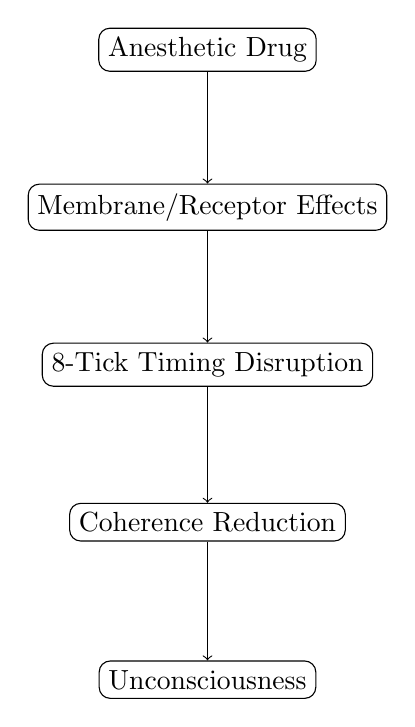
\begin{tikzpicture}[node distance=2cm, auto]
    \node[draw, rectangle, rounded corners] (drug) {Anesthetic Drug};
    \node[draw, rectangle, rounded corners, below of=drug] (membrane) {Membrane/Receptor Effects};
    \node[draw, rectangle, rounded corners, below of=membrane] (timing) {8-Tick Timing Disruption};
    \node[draw, rectangle, rounded corners, below of=timing] (coherence) {Coherence Reduction};
    \node[draw, rectangle, rounded corners, below of=coherence] (unconscious) {Unconsciousness};
    
    \draw[->] (drug) -- (membrane);
    \draw[->] (membrane) -- (timing);
    \draw[->] (timing) -- (coherence);
    \draw[->] (coherence) -- (unconscious);
\end{tikzpicture}
\end{center}

This explains:
\begin{itemize}
    \item Why chemically diverse drugs cause anesthesia (common target: coherence)
    \item The Meyer-Overton correlation (lipid solubility affects membrane timing)
    \item Why gamma oscillations (30-100 Hz) are suppressed (gamma = binding frequency)
\end{itemize}

\subsection{Method 1: Coherence-Based Anesthesia Monitoring}

\subsubsection{Coherence Index (CI) Calculation}

The invention defines a \textbf{Coherence Index (CI)} computed from multi-channel EEG:

\begin{equation}
\text{CI} = \frac{1}{N(N-1)} \sum_{i \neq j} \left| \langle e^{i(\phi_i(t) - \phi_j(t))} \rangle_t \right|
\end{equation}

where:
\begin{itemize}
    \item $\phi_i(t)$ is the instantaneous phase of channel $i$ in the gamma band
    \item $\langle \cdot \rangle_t$ denotes time averaging over a window
    \item $N$ is the number of electrode channels
\end{itemize}

\subsubsection{Consciousness Threshold}

Based on RS theory, the consciousness threshold is:

\begin{equation}
\text{CI}_{\text{threshold}} = 0.31
\end{equation}

This value corresponds to the Perturbational Complexity Index (PCI) threshold validated in clinical studies (Casali et al., 2013; Massimini et al., 2005).

\subsubsection{Monitoring Algorithm}

\begin{enumerate}
    \item Acquire multi-channel EEG (minimum 8 channels, preferably 32+)
    \item Filter for gamma band (30-100 Hz)
    \item Compute instantaneous phase using Hilbert transform
    \item Calculate CI over sliding windows (500 ms, 100 ms step)
    \item Compare CI to threshold:
    \begin{itemize}
        \item CI $> 0.5$: High consciousness risk (lighten anesthesia)
        \item CI $\in [0.31, 0.5]$: Transition zone (monitor closely)
        \item CI $< 0.31$: Unconscious (adequate anesthesia)
        \item CI $< 0.1$: Deep anesthesia (consider lightening)
    \end{itemize}
    \item Display real-time CI with trend and alerts
\end{enumerate}

\subsection{Method 2: Emergence Prediction}

\subsubsection{Pharmacokinetic-Coherence Model}

Combine drug concentration modeling with coherence dynamics:

\begin{equation}
\text{CI}(t) = \text{CI}_0 \cdot \exp\left(-k_{\text{drug}} \cdot C_{\text{eff}}(t)\right)
\end{equation}

where:
\begin{itemize}
    \item $\text{CI}_0$ is baseline coherence (awake)
    \item $k_{\text{drug}}$ is drug-specific coherence disruption constant
    \item $C_{\text{eff}}(t)$ is effect-site concentration
\end{itemize}

\subsubsection{Emergence Time Prediction}

Predict emergence by solving:

\begin{equation}
\text{CI}(t_{\text{emergence}}) = \text{CI}_{\text{threshold}}
\end{equation}

This gives:

\begin{equation}
t_{\text{emergence}} = t_{\text{stop}} + \frac{1}{k_e} \ln\left(\frac{C_{\text{eff}}(t_{\text{stop}})}{C_{\text{threshold}}}\right)
\end{equation}

where $C_{\text{threshold}}$ is the concentration corresponding to CI = 0.31.

\subsection{Method 3: Rational Anesthetic Drug Design}

\subsubsection{Design Criteria}

An ideal anesthetic should:
\begin{enumerate}
    \item Reduce coherence below threshold (CI $< 0.31$)
    \item Preserve basic neural function (not too deep: CI $> 0.05$)
    \item Have predictable coherence-concentration relationship
    \item Have minimal off-target effects
    \item Allow rapid recovery (coherence restoration)
\end{enumerate}

\subsubsection{Coherence-Disruption Screening Assay}

Screen candidate compounds using:

\begin{enumerate}
    \item \textbf{In vitro}: Measure effects on gamma oscillations in brain slices
    \item \textbf{Computational}: Model 8-tick phase disruption
    \item \textbf{In vivo}: Measure CI in animal models
\end{enumerate}

\subsubsection{Target Profile}

Optimal coherence-disruption profile:

\begin{equation}
k_{\text{drug}} \cdot C_{\text{therapeutic}} \approx \ln(2)
\end{equation}

This gives CI reduction to $\sim 0.5 \times \text{CI}_0$, ensuring unconsciousness without excessive depth.

\subsection{System Architecture}

\subsubsection{Hardware Components}

\begin{enumerate}
    \item \textbf{EEG Acquisition Module}
    \begin{itemize}
        \item 32+ channel amplifier
        \item Sampling rate $\geq$ 1000 Hz
        \item Common average reference
        \item Integrated impedance monitoring
    \end{itemize}
    
    \item \textbf{Processing Unit}
    \begin{itemize}
        \item Real-time DSP capability
        \item GPU for parallel phase calculations
        \item Low-latency output ($<$ 100 ms)
    \end{itemize}
    
    \item \textbf{Display Unit}
    \begin{itemize}
        \item Large numerical CI display
        \item Trend graph (last 60 minutes)
        \item Alert indicators (audible and visual)
        \item Integration with anesthesia machine
    \end{itemize}
\end{enumerate}

\subsubsection{Software Components}

\begin{enumerate}
    \item Real-time gamma-band filtering
    \item Hilbert transform phase extraction
    \item CI calculation engine
    \item Threshold comparison and alerting
    \item Drug concentration modeling (optional)
    \item Emergence prediction algorithm (optional)
    \item Data logging and reporting
\end{enumerate}

%==============================================================================
\section{CLAIMS}
%==============================================================================

\subsection{Independent Claims}

\begin{enumerate}[label=\textbf{Claim \arabic*:}, leftmargin=*]
    \item \textbf{A method for monitoring anesthesia depth}, comprising:
    \begin{enumerate}[label=(\alph*)]
        \item Acquiring multi-channel electroencephalogram (EEG) signals from a patient
        \item Filtering said signals to isolate gamma-band activity (30-100 Hz)
        \item Computing instantaneous phase of each channel using a transform
        \item Calculating a Coherence Index (CI) based on phase relationships between channels
        \item Comparing said CI to a predetermined threshold value
        \item Outputting an indication of anesthesia depth based on said comparison
    \end{enumerate}
    wherein said threshold value is derived from Recognition Science principles relating to the Gap-45 coherence boundary.

    \item \textbf{A system for real-time assessment of consciousness during anesthesia}, comprising:
    \begin{enumerate}[label=(\alph*)]
        \item An EEG acquisition module configured to receive signals from multiple electrodes
        \item A processing unit configured to:
        \begin{itemize}
            \item Filter signals for gamma-band frequencies
            \item Extract phase information from each channel
            \item Calculate a Coherence Index representing neural binding strength
        \end{itemize}
        \item A display unit configured to present CI values and consciousness state
        \item An alert module configured to signal when CI approaches consciousness threshold
    \end{enumerate}

    \item \textbf{A method for predicting emergence from anesthesia}, comprising:
    \begin{enumerate}[label=(\alph*)]
        \item Measuring Coherence Index (CI) during anesthesia
        \item Modeling drug concentration decay based on pharmacokinetics
        \item Computing the relationship between drug concentration and CI
        \item Predicting time to CI reaching consciousness threshold
        \item Outputting estimated emergence time
    \end{enumerate}

    \item \textbf{A method for designing anesthetic drugs}, comprising:
    \begin{enumerate}[label=(\alph*)]
        \item Identifying candidate compounds affecting neural membrane properties
        \item Measuring coherence disruption in a biological assay
        \item Calculating coherence-disruption constant $k_{\text{drug}}$
        \item Selecting compounds with optimal $k_{\text{drug}}$ profile
        \item Verifying unconsciousness induction at therapeutic concentrations
    \end{enumerate}
    wherein optimal profile is defined by CI reduction to below 0.31 at therapeutic dose without reduction below 0.05.

    \item \textbf{A device for measuring 8-tick neural synchronization}, comprising:
    \begin{enumerate}[label=(\alph*)]
        \item Multiple electrodes positioned to sample distinct brain regions
        \item Signal conditioning circuitry for gamma-band isolation
        \item Phase extraction circuitry implementing Hilbert transform
        \item Synchronization measurement circuitry computing inter-electrode phase coherence
        \item Output circuitry providing synchronization index
    \end{enumerate}
\end{enumerate}

\subsection{Dependent Claims}

\begin{enumerate}[label=\textbf{Claim \arabic*:}, leftmargin=*, resume]
    \item The method of Claim 1, wherein the threshold value is 0.31 $\pm$ 0.05.

    \item The method of Claim 1, wherein the transform is a Hilbert transform.

    \item The method of Claim 1, further comprising calculating a sub-threshold risk index based on CI proximity to threshold.

    \item The system of Claim 2, wherein the display unit provides color-coded indication:
    \begin{itemize}
        \item Green: CI $<$ 0.25 (adequate anesthesia)
        \item Yellow: CI $\in$ [0.25, 0.35] (transition zone)
        \item Red: CI $>$ 0.35 (consciousness risk)
    \end{itemize}

    \item The system of Claim 2, further comprising integration with drug delivery systems for closed-loop anesthesia control.

    \item The method of Claim 3, wherein pharmacokinetics include propofol, sevoflurane, or other common anesthetics.

    \item The method of Claim 4, wherein the biological assay comprises brain slice gamma oscillation measurement.

    \item The method of Claim 4, wherein the optimal $k_{\text{drug}}$ satisfies:
    \begin{equation}
    0.5 < k_{\text{drug}} \cdot C_{\text{therapeutic}} < 2.0
    \end{equation}

    \item The device of Claim 5, wherein the electrodes include at least 8 channels distributed across frontal, parietal, and occipital regions.

    \item A method for identifying intraoperative awareness risk, comprising:
    \begin{enumerate}[label=(\alph*)]
        \item Continuously monitoring CI during surgery
        \item Detecting CI excursions above 0.31
        \item Calculating cumulative time above threshold
        \item Flagging high-risk events for post-operative follow-up
    \end{enumerate}
\end{enumerate}

%==============================================================================
\section{ADVANTAGES OVER PRIOR ART}
%==============================================================================

\begin{enumerate}
    \item \textbf{Mechanistic basis}: Unlike BIS, the CI has a theoretical foundation explaining why it works.
    
    \item \textbf{Universal applicability}: Works for all anesthetic classes because all disrupt coherence.
    
    \item \textbf{Individual precision}: Measures actual brain state, not population-averaged drug response.
    
    \item \textbf{Emergence prediction}: Pharmacokinetic-coherence model enables accurate timing.
    
    \item \textbf{Drug design guidance}: Provides rational criteria for new anesthetic development.
    
    \item \textbf{Awareness prevention}: Early detection of consciousness risk.
\end{enumerate}

%==============================================================================
\section{INDUSTRIAL APPLICABILITY}
%==============================================================================

The invention has applications in:

\begin{enumerate}
    \item \textbf{Clinical anesthesia}: Improved monitoring in operating rooms
    \item \textbf{Intensive care}: Sedation depth assessment
    \item \textbf{Pharmaceutical industry}: Rational anesthetic drug design
    \item \textbf{Medical devices}: New class of consciousness monitors
    \item \textbf{Research}: Tools for studying consciousness mechanisms
\end{enumerate}

%==============================================================================
\section{ABSTRACT}
%==============================================================================

A method and system for monitoring anesthesia depth based on neural coherence as defined by Recognition Science. The invention measures a Coherence Index (CI) derived from gamma-band EEG phase synchronization across brain regions. A CI threshold of approximately 0.31 demarcates conscious from unconscious states. The system provides real-time monitoring, emergence prediction, and guidance for rational anesthetic drug design. By targeting the fundamental mechanism of anesthetic action---disruption of coherent neural binding---the invention offers advantages over empirical methods such as BIS monitoring. Applications include clinical anesthesia monitoring, intensive care sedation assessment, and pharmaceutical development of safer anesthetics with predictable coherence-disruption profiles.

%==============================================================================
\section{INVENTOR DECLARATION}
%==============================================================================

I, Jonathan Washburn, declare that I am the inventor of the subject matter claimed herein, that this application is the first application for patent on this invention, and that I have read and understand the contents of this specification and claims.

\vspace{2em}

\noindent\textbf{Signature:} \rule{5cm}{0.4pt}

\noindent\textbf{Date:} January 18, 2026

\noindent\textbf{Email:} washburn.jonathan@gmail.com

\end{document}
